% !TEX TS-program = lualatex
% !TEX encoding = UTF-8 Unicode
% !TEX spellcheck = de_DE
% © 2017-2024 Moritz Brinkmann, CC-by-sa
% https://ma.latexkurs.de

\documentclass[
	vorläufig=false,
	datum=2023-02-17,
	titel={erster Tag},
%	web=true, handout,
	kursA,
]{../tex/latexkurs-slides}

\usepackage{caption,booktabs,siunitx,adjustbox}

\setotherlanguages{russian,dutch}


%% Notes:
%% Zitate: Harvard-Methode (AuthorYear)


\begin{document}

\begin{frame}{Lernziele}
Nach den zwei Workshop-Tagen können Sie …
\begin{itemize}
\item einfache Dokumente in \LaTeX\ setzen
\item Hilfestellungen in Klassen- und Paketdokumentationen auffinden
\item mehrsprachige Dokumente erstellen
\item Abbildungen einbinden und Tabellen anlegen
\item Referenzapparate erzeugen
\item mathematische Formeln setzen
\item größere Projekte strukturieren
\end{itemize}
\end{frame}

\begin{frame}<handout:0>[t]{Organisatorisches}%{Allgemeines}
	\begin{block}<1->{Termine}
		\begin{itemize}
			\item	zwei Sitzungen:
				\begin{itemize}
				\kursAB{
					\item Samstag 17. Februar (heute)
					\item Sonntag 18. Februar (morgen)
				}{
					\item Samstag 2. März (heute)
					\item Sonntag 3. März (morgen)
				}
				\end{itemize}
			jeweils 10 bis 15 Uhr
			\item ca. 45 Minuten Pause
		\end{itemize}
	\end{block}
	\begin{block}<2>{Materialien}
		\begin{columns}
			\column{.7\textwidth}
				\begin{itemize}
					\item Alle Materialien stehen auf der \href{https://ma.latexkurs.de}{Workshophomepage} oder im \href{https://ilias.uni-mannheim.de/goto.php?target=fold_1461908&client_id=ILIAS}{ILIAS} zum Download:\\[1ex]
					\url{https://ma.latexkurs.de/}\\\quad
				\end{itemize}
			\column{.25\textwidth}
				\vspace*{-2mm}
				
				\begin{minipage}{1.05in}
					\centering
					\textcolor{white}{\rule{0.9in}{0.9in}}\vspace*{-0.86in}
					\qrcode{https://ma.latexkurs.de}
				\end{minipage}
			\end{columns}
	\end{block}
\end{frame}

\begin{frame}<all:0| handout:99>[t]{Organisatorisches}%{Allgemeines}
	\begin{block}{Termine}
		\begin{itemize}
			\item zwei Sitzungen je Termin:
			\vspace*{-1.2ex}
				\begin{columns}
					\column{0.26\textwidth}
					\begin{itemize}\setlength{\itemsep}{0pt}
							\item Samstag 17. Februar
							\item Sonntag 18. Februar
					\end{itemize}
					\column{0.04\textwidth}
						\emph{oder}
					\column{0.26\textwidth}
					\begin{itemize}\setlength{\itemsep}{0pt}
						\item Samstag 2. März
						\item Sonntag 3. März
					\end{itemize}
					\column{0.1\textwidth}
						\vspace{1.5cm}
				\end{columns}
%				\vspace{1ex}
			\item jeweils 10 bis 15 Uhr
			\item ca. 45 Minuten Pause
		\end{itemize}
	\end{block}
	\begin{block}{Materialien}
		\begin{columns}
			\column{.7\textwidth}
				\begin{itemize}
					\item Alle Materialien stehen auf der \href{https://ma.latexkurs.de}{Workshophomepage} oder im \href{https://ilias.uni-mannheim.de/goto.php?target=fold_1461908&client_id=ILIAS}{ILIAS}
					 zum Download:\\[1ex]
					\url{https://ma.latexkurs.de/}\\[1em]\quad
				\end{itemize}
			\column{.25\textwidth}
				\vspace*{-2mm}
				
				\begin{minipage}{1.05in}
					\centering
					\textcolor{white}{\rule{0.9in}{0.9in}}\vspace*{-0.86in}
					\qrcode{https://ma.latexkurs.de}
				\end{minipage}
			\end{columns}
	\end{block}
\end{frame}

\begin{frame}[t]{Organisatorisches}
	\begin{block}{Übungen}
		\begin{itemize}
			\item Theorie und Praxisphasen wechseln sich ab.
			\item Sie dürfen (und sollen) Beispiele \emph{jederzeit} selbst an Ihrem Computer nachmachen.
			\item Probieren Sie Neues ruhig \emph{sofort} aus …!
			\item Fragen Sie gerne nach, wenn Sie etwas nicht hinkriegen.
			\item Falls Sie \href{https://www.overleaf.com?r=60500875&rm=d&rs=b}{Overleaf} nutzen können Sie Ihren Quellcode bei Fragen mit \href{mailto:overleaf@latexkurs.de}{\texttt{overleaf@latexkurs.de}} teilen.
		\end{itemize}
	\end{block}
%	\begin{olcol}
		\begin{block}{\LaTeX\ flavour}
			Die Inhalte dieses Kurses beziehen sich auf die (relativ moderne) Variante \hologo{LuaLaTeX}.
		\end{block}
%	\end{olcol}
%	\overleaf{tex00}
\end{frame}


\begin{frame}[t,allowframebreaks]{Inhalt}
	\tableofcontents
\end{frame}

%%%%%%%%%%%%%%%%%%%%%%%%%%%%%%%%%%%%%%%%%%%%%%%%%%%%%%%%%%%%%%%%%%%%%%%%%%%%%%%%%%%%%%%%%%%%%%%%%%%%%%%%%%
\teil[Worum geht es überhaupt?]{The Name of the Game}
%%%%%%%%%%%%%%%%%%%%%%%%%%%%%%%%%%%%%%%%%%%%%%%%%%%%%%%%%%%%%%%%%%%%%%%%%%%%%%%%%%%%%%%%%%%%%%%%%%%%%%%%%%
\subsection*{\TeX}

\begin{frame}[<+->][t]{The Name of the Game}
	\begin{itemize}
		\item Programm \alert{\TeX} (Seit 1977)
			\only<1>{\\ Geschrieben von Donald E. Knuth für sein Buch\\„The Art of Computer Programming“.
			\\ „\TeX“ von griechisch τέχνη} % téchne, altgr. Fähigkeit, Kunstfertigkeit, Handwerk
		\item Makropaket \alert{plain}\TeX
			\only<2>{\\ Macht \TeX\ für normale Nutzer bedienbar.}
		\item großes Makropaket \alert{La}\TeX\ (Anfänge 1980er)
			\only<3>{\\ Von Leslie Lamport: „Lamport’s \TeX“.\\ Viele Vereinfachungen für den normalen Anwender.}
		\item aktuelle, stabile Version: \alert{La}\TeX\,\alert{2$_\varepsilon$} (1994)
			\only<4>{\\ „in einer $\varepsilon$-Umgebung von 2“}
		\item zukünftige Entwicklung: \LaTeX{}3 \\ noch nicht eigenständig verfügbar, aber als Paket \texttt{expl3} in \LaTeXe%\\ (bietet \LaTeX{}3-Syntax für Paketautoren)
	\end{itemize}		
\end{frame}

\begin{frame}[t]{Was ist \TeX\ – und was nicht?}
	\only<1>{
		\begin{block}{Dafür ist \LaTeX{} gut geeignet …}
			\begin{itemize}
				%\item Programm, um „The Art of Computer Programming“ zu schreiben
				\item Alle Schriftstücke mit logischem Aufbau
				\begin{itemize}
					\item Naturwissenschaftliche Arbeiten (hervorragender Mathesatz)
					\item Geisteswissenschaftliche Arbeiten (hervorragende Mehrsprachigkeit, Bibliographieerstellung, 	Erstellung von Apparaten etc.)
					\item Artikel, Bachelorarbeiten, Dissertationen, …
					\item Buchreihen, Briefe
					\item Präsentationen
				\end{itemize}
				\item Viel „Missbrauch“ durch kreative Paketautoren
			\end{itemize}
		\end{block}
	}\only<2>{
		\begin{block}{Dafür ist \LaTeX{} weniger gut geeignet …}
			\begin{itemize}
				\item Dokumente ohne logische Struktur
				\begin{itemize}
					\item Präsentationen (bunt, drehend, blinkend, „durcheinander“)
					\item Werbezettel
					\item Plakate 
				\end{itemize}
				\item Dokumente mit vielen uneinheitlichen Bildern, die frei bewegt werden
			\end{itemize}
		\end{block}
	}
\end{frame}

\begin{frame}{Wie funktioniert \TeX?}
	\begin{itemize}
		\item WYSIWYM
		\item reine Textdateien
		\item keine versteckten Einstellungen
		\item Textauszeichnung durch besondere Befehle:
		\begin{itemize}
			\item „Ich will einen Artikel schreiben!“
			\item „Setze eine Überschrift!“
			\item „Schreibe das folgende fett!“
			\item „Setze eine Tabelle, die …“
		\end{itemize}
	\end{itemize}
\end{frame}

\begin{frame}[t]{Wie funktioniert \TeX?}
	\begin{columns}[t]
		\begin{column}{.45\textwidth}
			\begin{block}{Vorteile}
				\begin{itemize}
					\item Stabilität und Portabilität
					\item geringe Dateigrößen
					\item Bearbeitung mit beliebigem Editor
					\item Textdateien \emph{immer} lesbar
					\item Ausgabe überall gleich
				\end{itemize}
			\end{block}
		\end{column}
		\begin{column}{.45\textwidth}
			\begin{block}{Nachteile}
				\begin{itemize}
					\item Ergebnis nicht direkt sichtbar
					\item unintuitive Bedienung
					\item steile Lernkurve
					\item Bei Änderungen muss alles neu kompiliert werden
					\item komplizierte Layout-wünsche schwer realisierbar
				\end{itemize}
			\end{block}
		\end{column}
	\end{columns}
\end{frame}
	

\begin{frame}[fragile]{Ein einfaches \TeX-Dokument}
	Wie lässt sich Text von Befehlen unterscheiden?\\[1em]
	
	Ansatz in \emph{klassischen} Programmiersprachen:
\begin{lstlisting}
print ( “ Hallo Welt! ” );
\end{lstlisting}
	⇒ für ein Textsatzprogramm ungeeignet
\end{frame}
\begin{frame}[fragile]{Ein einfaches \TeX-Dokument}
	\begin{itemize}
		\item \TeX{} ist eine Auszeichnungssprache (\emph{markup language})
		\item einzelne Zeichen haben besondere Bedeutung
		\item Backslash (\verb|\|) dient als \emph{escape character} und markiert den Anfang eines Befehls: \verb|\chapter \section \author|
	\end{itemize}\quad\\[1em]
	Einfachstes \TeX-Dokument:
\begin{lstlisting}
Hallo Welt! \bye 
\end{lstlisting}\quad\\[1em]
	\pause
	\promt|tex dokument.tex|\\ erzeugt ein |.dvi|-Dokument und eine |.log|-Datei
	% Live-Vorführung
\end{frame}

\begin{frame}[fragile]{Ein einfaches \LaTeX-Dokument}
\begin{LTXexample}
\documentclass{minimal}
\begin{document}
Hallo Welt!
\end{document}
\end{LTXexample}
\pause\vfill
\begin{arbeitsauftrag}
Erstellen Sie ein erstes \LaTeX-Dokument, indem Sie dieses Minimalbeispiel in Ihrem Editor abtippen!
\end{arbeitsauftrag}
\end{frame}

\begin{frame}[fragile]{Befehlszeichen}
	\begin{tabular}{ll}
			\verb|\| & \emph{escape character}, Leitet Befehle ein \\
			\verb|{}| & \emph{grouping character}, gruppieren zusammengehörende Zeichen \\& z.\,B. Argumente \verb|\textbf{fett}|\\
			\verb|$| & \emph{math character}, startet und beendet Mathemodus \\
			\verb|&| & \emph{tabbing character}, trennt Spalten in Tabellen \\
			\verb|%| & \emph{comment character} Kommentiert den Rest der Zeile aus \\
			\verb|^_~#| & weitere Zeichen mit besonderer Bedeutung
	\end{tabular}
\end{frame}

%%%%%%%%%%%%%%%%%%%%%%%%%%%%%%%%%%%%%%%%%%%%%%%%%%%%%%%%%%%%%%%%%%%%%%%%%%%%%%%%%%%%%%%%%%%%%%%%%%%%%%%%%%
\teil{Grundlegende Bedienung}
%%%%%%%%%%%%%%%%%%%%%%%%%%%%%%%%%%%%%%%%%%%%%%%%%%%%%%%%%%%%%%%%%%%%%%%%%%%%%%%%%%%%%%%%%%%%%%%%%%%%%%%%%%
\subsection{Klassen und Pakete}
\subsubsection*{Dokumentenklassen}

\begin{frame}{Dokumentenklassen}
	Dokumentenklassen legen grundlegende Eigenschaften des Dokuments fest:
	\begin{itemize}
		\item Layout
		\item Standardschriften
		\item Satzspiegel
		\item Gliederungsbefehle
		\item Aussehen von Verzeichnissen, Tabellen, Aufzählungen, …
	\end{itemize}
	Eigenschaften sind durch Änderung von Optionen oder Laden von Paketen anpassbar.
\end{frame}

\begin{frame}{Dokumentenklassen}
	\begin{tabular}{rl}
		&\kern-1.5cm \bf Standardklassen\\
		article & (Kurze) Artikel\\
		report & Reporte, Tagungsberichte\\
		book & Bücher\\
		letter & Briefe\\
		minimal & für Minimalbeispiele\\ \\
		&\kern-1.5cm \bf KOMA-Script\\
		scrartcl & Erweiterung von article\\
		scrreprt & Erweiterung von report\\
		scrbook & Erweiterung von book\\
		scrlttr2 & sehr mächtige Briefklasse\\ \\
		&\kern-1.5cm \bf Spezialklassen\\
		beamer & für Präsentationen\\
		tikzposter & wissenschaftliche Poster
	\end{tabular}
\end{frame}

\subsubsection*{Pakete}
\begin{frame}[fragile]{Pakete}
\begin{itemize}
\item Pakete bieten zusätzliche Funktionalität
\item Arbeitserleicherungen
\item Fehlerkorrekturen
\item Einbinden in der Präambel mittels
%\pdfmarginpar[Help]{Die Praeambel ist alles was zwischen documentclass{} und begin{document} steht}
|\usepackage[|\meta{option(en)}|]{|\meta{paketname}|}|:
\begin{lstlisting}
\documentclass{article}
\usepackage{
  amsmath,
  hyperref,
}
\usepackage[left=2cm]{geometry}
\end{lstlisting}
\end{itemize}
\end{frame}

\begin{frame}[fragile]{Gliederungsbefehle}
	\begin{itemize}
		\item Gliederungen strukturieren Dokumente
		\item ermöglichen automatische Nummerierung, Eintragung in Verzeichnisse, Kolumnentitel etc.
		\item Werden von der Dokumentenklasse festgelegt
		\item Grundstruktur im Kernel definiert
		\item[⇒] bestimmte Elemente immer verfügbar
	\end{itemize}
	\vfill
	\begin{olcol}
\begin{lstlisting}
\part{Band I}
\chapter{Kapitel}
\section{Abschnitt}
\subsection{Unterabschnitt}
\subsubsection{Unterunterabschnitt}
\paragraph{Paragraph}
\subparagraph{Unterparagraph}
\end{lstlisting}
	\end{olcol}
	\overleaf*{tex01}
\end{frame}


%\begin{frame}{Kleine Auswahl an Paketen}
%	\begin{tabular}{rl}
%		graphics/x & bietet (erweiterte) Grafikunterstützung\\
%		amsmath & Verbesserungen, Erweiterungen für den Mathesatz\\
%		babel/polyglossia & Spachrensupport (Umbruchregeln, …)\\
%		inputenc & ermöglicht verschiedene Eingabekodierungen\\
%		fontenc & ermöglicht verschiedene Fontkodierungen\\
%		lmodern & Stellt auf die lmodern-Schriften um\\
%		fontspec & ermöglicht Nutzung von Systemschriften\\
%		tikz & sehr mächtige Zeichenumgebung\\
%		\vdots & \vdots
%	\end{tabular}
%\end{frame}


\begin{frame}[c,fragile]{Grundbefehle}{allgemein}
\begin{tabular}{ll}
|\textrm{Serifen}| & \textrm{Serifen \quad Abcdxyz}\\
|\textit{kursiv}| & \textrm{\textit{kursiv \quad Abcdxyz}} \\%(\emph{nicht} |{\it kursiv}| verwenden)\\
%|\textsl{geneigt}| & \textrm{\textsl{geneigt \quad Abcdxyz}}\\
|\textsf{serifenlos}| & \textsf{serifenlos \quad Abcdxyz}\\
|\textbf{fett}| & \textbf{fett \quad Abcdxyz}\\
|\texttt{Schreibmaschine}| & \texttt{Schreibmaschine \quad Abcdxyz}\\
|\textsc{Kapitälchen}| & \textsc{Kapitälchen \quad Abcdxyz}\\
|\emph{Hervorhebung}| & \emph{Hervorhebung \quad Abcdxyz}\\
|\\| & Zeilenende\\
|\par| oder Leerzeile & Absatzende\\
|$E = \frac{p^2}{2m}$| & Inline-Mathemodus: $E = \frac{p^2}{2m}$\\
|\[E = \frac{p^2}{2m}\]| & Display-Mathemodus: $\displaystyle E = \frac{p^2}{2m}$\\ % Arno: „well that’s cheated …“ ;-)
|\tableofcontents| & Produziert Inhaltsverzeichnis\\
|\today| & aktuelles Datum
\end{tabular}
\overleaf{tex01}
\end{frame}

\subsection{Grundbefehle}

\begin{frame}[c,fragile]{Grundbefehle}{Schriftgrößen}
\begin{tabular}{ll}
|\tiny| & \tiny winzig \\
|\small| & \small klein \\
|\normalsize| & \normalsize normal\\
|\large| & \large groß\\
|\Large| & \Large größer\\
|\LARGE| & \LARGE noch größer\\
|\huge| & \huge riesig\\
|\Huge| & \Huge noch riesiger\\
\end{tabular}
%Manuelle Anpassung: |\fontsize{10}{12}\selectfont|
\overleaf{tex01}
\end{frame}

\begin{frame}[c]{Hilfsdateien}
	\begin{tabular}{ll}
		& \bf Eingabe\\
		.tex & \TeX-Datei mit Dokumententext\\ \\
		& \bf Ausgabe\\
		.pdf & pdf\TeX-Ausgabe oder Umwandlung von (x)dvi\\ \\\pause
		& \bf Hilfsdateien (nur schreiben)\\
		.log & Log-Datei mit Informationen, Warnungen, Fehlern\\ \\\pause
		& \bf Hilfsdateien (schreiben und lesen)\\
		.aux & Hilfsdatei mit temporären Informationen\\
		.toc & table of contents\\
		.lof & list of figures\\
		.synctex.gz & nötig für die Sync\TeX-Funktion\\
		\vdots & \vdots
	\end{tabular}
\end{frame}


%\subsection{Engines und Formate}
%\begin{frame}{\TeX-Engines und -Formate}{Begriffsbildung}
%	\begin{description}
%		\item[engine] Das Programm, das die eigentliche Satz-Arbeit macht:\\\TeX, \hologo{pdfTeX}, \luaTeX
%		\item[format] Große Sammlung von Makros, die die Arbeit erleichtern sollen:\\plain\TeX, \LaTeX, \hologo{ConTeXt}
%		\item[distribution] Bundle von Engines, Formaten, Erweiterungen (Paketen, Modulen) und Hilfsprogrammen:\\\TeXlive, Mac\TeX, \MikTeX
%	\end{description}
%\end{frame}
%
%\begin{frame}{\TeX-Engines und -Formate}{Wichtige Engines}
%	\begin{description}
%		\item[\TeX] Das ursprüngliche, von Donald E. Knuth geschriebene Programm.
%		\item[\hologo{pdfTeX}] Engine, die direkt PDF-Dateien schreiben kann\\Ermöglicht viele PDF-spezifische Features wie z.\,B. Mikrotypografie.
%		\item[\XeTeX] Verarbeitet standardmäßig utf8-Encoding, bietet die Möglichkeit, Systemschriften zu benutzen und die Textrichtung einfach zu ändern.
%		\item[\luaTeX] Bietet quasi alles was \XeTeX kann und enthält die Skriptsprache Lua, die man aus dem \TeX-Dokument heraus aufrufen kann.
%	\end{description}
%\end{frame}
%
%\begin{frame}[fragile]{\TeX-Engines und -Formate}{Programm\/namen}
%	Ausgeführtes Programm bestimmt Engine und Format:\\[1em]
%	\begin{description}
%		\item[|pdftex|] \hologo{pdfTeX}-Engine, plain-Format
%		\item[|pdflatex|] \hologo{pdfTeX}-Engine, \LaTeXe-Format
%		\item[|latex|] \hologo{pdfTeX}-Engine, \LaTeXe-Format, DVI-Output
%		\item[|xelatex|] \XeTeX-Engine, \LaTeXe-Format
%		\item[|lualatex|] \luaTeX-Engine, \LaTeXe-Format, PDF-Output
%	\end{description}
%\end{frame}

%%%%%%%%%%%%%%%%%%%%%%%%%%%%%%%%%%%%%%%%%%%%%%%%%%%%%%%%%%%%%%%%%%%%%%%%%%%%%%%%%%%%%%%%%%%%%%%%%%%%%%%%%%
\teil{Typografische Grundlagen}
%%%%%%%%%%%%%%%%%%%%%%%%%%%%%%%%%%%%%%%%%%%%%%%%%%%%%%%%%%%%%%%%%%%%%%%%%%%%%%%%%%%%%%%%%%%%%%%%%%%%%%%%%%
\subsection{Makrotypografie}

\begin{frame}{Makrotypografie}
	\begin{itemize}
		\item Satzspiegel
		\item Kopf und Fußzeilen
		\item Wahl der Schriften
		\item Formatierung von Abständen
		\item Aussehen von Verzeichnissen, Fußnoten, …
	\end{itemize}
	
	\pause
	\begin{olcol}
		\begin{arbeitsauftrag}
			Laden Sie sich die Datei \href{https://latexkurs.github.io/MA-de/uebung_layout.tex}{\texttt{uebung\_layout.tex}} von der Workshopwebseite herunter. Vollziehen Sie daran nach und nach alle typografischen Einstellungen, die besprochen werden.
		
			Im Idealfall wählen Sie alle Werte so, dass Sie den Anforderungen an die Ihnen bevorstehende Abschlussarbeit genügen.
		\end{arbeitsauftrag}
	\end{olcol}
	\overleaf{tex02}
\end{frame}

\begin{frame}{Vorgaben für VWL-Bachelorarbeiten}
\begingroup
\renewcommand{\familydefault}{\rmdefault}
\begin{fancyquote}
\vspace{-1ex}
\normalfont\textbf{\Large Style}
\begin{description}[Left and right margin]
\item[Format] one-sided DIN A4
\item[Font Size] \SI{12}{pt}
\item[Line Spread] \SI{1.5}{pt}
\item[Alignment] justified (“Blocksatz”)
\item[Left and right margin] \SI{3}{\centi\meter}
\end{description}
\quoted{\itshape \href{https://www.vwl.uni-mannheim.de/media/Fakultaeten/vwl/Dokumente/20141105_Guidelines.pdf}{Guidelines for Bachelor theses}}
\end{fancyquote}
\endgroup
\end{frame}

\begin{frame}{Der Satzspiegel}
	Mit Satzspiegel bezeichnet man die vom Text bedeckte Fläche (im Gegensatz zu den Rändern)
	\begin{itemize}
		\item Ein- oder zweiseitiger Satz?
		\item Schriftgröße, Laufweite,
		\item Kopf- und Fußzeilen
		\item Textspalten
	\end{itemize}
\end{frame}


\begin{frame}{Moderne Satzspiegelkonstruktion}
	\centering \small
	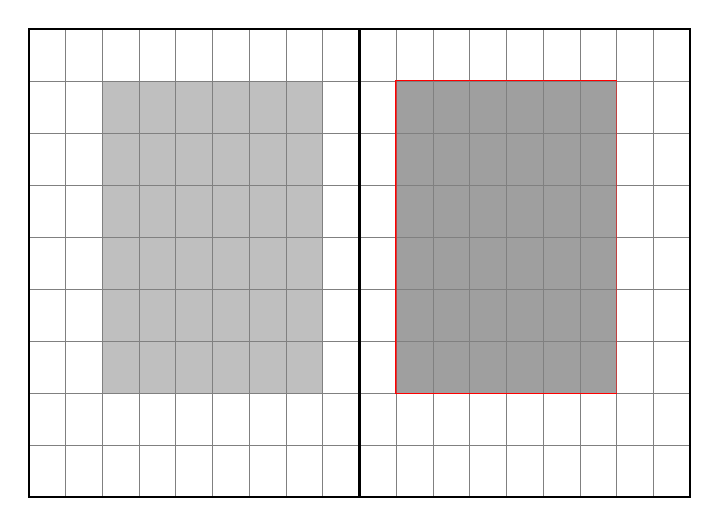
\begin{tikzpicture}
		\coordinate (a) at (-4.20, 5.95);
		\coordinate (b) at ( 0.00, 5.95);
		\coordinate (c) at ( 4.20, 5.95);
		\coordinate (d) at (-4.20, 0.00);
		\coordinate (e) at ( 0.00, 0.00);
		\coordinate (f) at ( 4.20, 0.00);
		
		\coordinate (A2) at ( 0.464, 5.29);
		\coordinate (D2) at ( 3.266, 1.32);
		\coordinate (A2’) at (-0.464, 5.29);
		\coordinate (D2’) at (-3.266, 1.32);

		\draw<1-2>[help lines, xstep=8.4/18, ystep=11.9/18] (a) grid (f);
		
		\draw<2>[red, fill=gray, fill opacity=.5] (A2) rectangle (D2);
		\fill<3>[gray, fill opacity=.5] (A2) rectangle (D2);
		\fill<3>[gray, fill opacity=.5] (A2’) rectangle (D2’);

		\draw [thick]
			(a) rectangle (e)
			(b) rectangle (f);
	\end{tikzpicture}
\end{frame}
%% Markus Kohm: „Satzspiegelkonstruktionen im Vergleich“ http://www.dante.de/tex/Dokumente/KohmSatzspiegel.pdf

\begin{frame}{Satzspiegel bei Gutenberg}
	\hspace{7.00cm}\includegraphics[height=5.95cm]{gutenbergbibel}
\end{frame}

\begin{frame}[fragile]{Satzspiegel mit KOMA-Skript}
\begin{itemize}
	\item KOMA-Skript bietet optimale Satzspiegelkonstruktion mittels eigenem Paket \pkg{typearea}
	\item Anpassung eigentlich nur bei besonders breiten oder engen Schriften nötig:
	\\Option |DIV=|\meta{Faktor}
	\\Autom. Berechnung anhand der Seitengröße: |DIV=calc| 
	\\Berechnung nach mittelalterl. Buchseitenkanon: |DIV=classic|
	\item Bindekorrektur mittels Option |BCOR=|\meta{Länge}
\end{itemize}
\begin{lstlisting}
\documentclass[DIV=9, BCOR=12mm]{scrbook}
\end{lstlisting}
\vfill
\begin{olcol}
Bei Nicht-KOMA-Klassen muss |typearea| direkt geladen werden:
\begin{lstlisting}
\usepackage[DIV=13, BCOR=2cm]{typearea}
\end{lstlisting}
\end{olcol}
\end{frame}

\begin{frame}[fragile]{Satzspiegel mit |geometry|}
Paket \pkg{geometry}  erlaubt manuelle Einstellung des Satzspiegels:
\begin{lstlisting}
\usepackage[top=2cm, bottom=5cm]{geometry}
\end{lstlisting}
oder:
\begin{lstlisting}
\usepackage{geometry}
\geometry{top=2cm, bottom=5cm}
\end{lstlisting}
\end{frame}


\begin{frame}[fragile,t]{Satzspiegel mit |geometry|}
\begin{block}{mögliche Optionen}
	\vspace{-1em}
\begin{verbatim}
paper
left, right, inner, outer, hmargin
top, bottom, vmargin
margin
bindingoffset, textwidth, textheight
twocolumn, columnsep, marginparsep, footnotesep
headsep, footsep, nofoot, nohead
hoffset, voffset, offset
includehead, includefoot
\end{verbatim}
\end{block}
%\pause
%\begin{arbeitsauftrag}
%Stellen Sie in Ihrem Dokument Ränder links und rechts von \SI{3}{\centi\meter} ein.
%\end{arbeitsauftrag}
\end{frame}

\begin{frame}[fragile]{Zeilenabstand}
Paket \pkg{setspace} erlaubt Anpassung der Zeilenabstände:
\begin{lstlisting}
\usepackage{setspace}
\singlespacing
\onehalfspacing
\doublespacing
\end{lstlisting}
Abstand in Fußnoten, etc. bleibt dabei gleich.\\
Finetuning: |\setstretch{|\meta{Faktor}|}|
%\pause
%\begin{arbeitsauftrag}
%Vergrößern Sie den Zeilenabstand Ihres Dokuments auf \num{1.5}.
%\end{arbeitsauftrag}
\end{frame}



\subsubsection*{Kopf- und Fußzeilen}
\begin{frame}[fragile, t]{Kopf- und Fußzeilen}
	\begin{itemize}
		\item Kopf- und Fußzeilen enthalten wichtige Informationen über das Dokument 
		\begin{itemize}
			\item lebende Kolumnentitel
			\item Seitenzahlen
		\end{itemize}
		\item Anpassung mittels verschiedener Pakete
		\item Auswahl über |\pagestyle{|\meta{Seitenstil}|}| oder |\thispagestyle{|\meta{Seitenstil}|}| 
		\item Voreinstellungen: |empty|, |plain|, |headings|
	\end{itemize}
\overleaf{tex03}
\end{frame}


\begin{frame}[fragile, t]{Kopf- und Fußzeilen mit scrlayer-scrpage}%
\kern-.7ex Paket definiert zwei Seitenstile: |scrheadings| und |screadings.plain|

Anpassung mittels z.\,B.\\|\lehead[|\meta{Inhalt plain.scrheadings}|]{|\meta{Inhalt scrheadings}|}|

\begin{center}\vspace{-1em}\small
\begin{tikzpicture}
		\coordinate (a) at (-.5\textwidth, 3.50);
		\coordinate (b) at ( 0.00, 3.50);
		\coordinate (c) at ( .5\textwidth, 3.50);
		\coordinate (d) at (-.5\textwidth, 2.70);
		\coordinate (e) at ( 0.00, 2.70);
		\coordinate (f) at ( .5\textwidth, 2.70);
		\coordinate (g) at (-.5\textwidth, 0.80);
		\coordinate (h) at ( 0.00, 0.80);
		\coordinate (i) at ( .5\textwidth, 0.80);
		\coordinate (j) at (-.5\textwidth, 0.00);
		\coordinate (k) at ( 0.00, 0.00);
		\coordinate (l) at ( .5\textwidth, 0.00);

		\node (A) at (-3/8*\textwidth, 3.00) {\color{red}|\lehead|};
		\node (B) at (-2/8*\textwidth, 3.00) {\color{green}|\cehead|};
		\node (C) at (-1/8*\textwidth, 3.00) {\color{blue}|\rehead|};
		\node (D) at ( 1/8*\textwidth, 3.00) {\color{blue}|\lohead|};
		\node (E) at ( 2/8*\textwidth, 3.00) {\color{green}|\cohead|};
		\node (F) at ( 3/8*\textwidth, 3.00) {\color{red}|\rohead|};
		
		\node (G) at (-3/8*\textwidth, 0.50) {\color{red}|\lefoot|};
		\node (H) at (-2/8*\textwidth, 0.50) {\color{green}|\cefoot|};
		\node (I) at (-1/8*\textwidth, 0.50) {\color{blue}|\refoot|};
		\node (J) at ( 1/8*\textwidth, 0.50) {\color{blue}|\lofoot|};
		\node (K) at ( 2/8*\textwidth, 0.50) {\color{green}|\cofoot|};
		\node (L) at ( 3/8*\textwidth, 0.50) {\color{red}|\rofoot|};

\only<2>{
		\node (M) at ( 0, 2.6) {\color{blue}\texttt{\textbackslash ihead}};
		\node (N) at ( 0, 2.3) {\color{green}\texttt{\textbackslash mhead}};
		\node (O) at ( 0, 2.0) {\color{red}\texttt{\textbackslash ohead}};
		
		\node (P) at ( 0, 0.9) {\color{blue}\texttt{\textbackslash ifoot}};
		\node (Q) at ( 0, 1.2) {\color{green}\texttt{\textbackslash mfoot}};
		\node (R) at ( 0, 1.5) {\color{red}\texttt{\textbackslash ofoot}};
		
		\draw [red, smooth, out=270, in=180] (A.south) to (O.west);
		\draw [red, smooth, out=0, in=270]	(O.east) to (F.south);
		\draw [green, smooth, out=270, in=180] (B.south) to (N.west);
		\draw [green, smooth, out=0, in=270]	(N.east) to (E.south);
		\draw [blue, smooth, out=270, in=180] (C.south) to (M.west);
		\draw [blue, smooth, out=0, in=270]	(M.east) to (D.south);
		
		\draw [red, smooth, out=90, in=180] (G.north) to (R.west);
		\draw [red, smooth, out=0, in=90]	(R.east) to (L.north);
		\draw [green, smooth, out=90, in=180] (H.north) to (Q.west);
		\draw [green, smooth, out=0, in=90]	(Q.east) to (K.north);
		\draw [blue, smooth, out=90, in=180] (I.north) to (P.west);
		\draw [blue, smooth, out=0, in=90]	(P.east) to (J.north);
}
		\draw [thick]
			(d) -- (a) -- (c) -- (f)
			(g) -- (j) -- (l) -- (i)
			(b) -- (e)
			(h) -- (k);
		\draw [thick, dashed]
			(d) -- (g)
			(f) -- (i);
		\draw<1>[thick, dashed] (e) -- (h);
\end{tikzpicture}
\end{center}\vspace{-.5em}

\begin{lstlisting}
\documentclass{scrartcl}
\usepackage{scrlayer-scrpage}
\lohead*{Peter Musterheinzel}
\rohead*{Seitenstile mit KOMA-Script}
\pagestyle{scrheadings}
\end{lstlisting}
\end{frame}


%% todo: inputenc/notwendigkeit von xelatex erklären?

%\begin{frame}[fragile]{Eingabekodierung}
%\begin{itemize}
%\item Früher\texttrademark\pdfmarginpar{Früher heißt hier in den 60er und 70er Jahren.} hat man Buchstaben mit 7\,bit gespeichert\\
%z.\,B. ASCII-Zeichensatz:
%\begin{verbatim*}
% !"#$%&'()*+,-./0123456789:;<=>?
%@ABCDEFGHIJKLMNOPQRSTUVWXYZ[\]^_
%`abcdefghijklmnopqrstuvwxyz{|}~ 
%\end{verbatim*}
%\item<2-> \hologo{pdfLaTeX} geht von ASCII-Kodierung aus und versteht normalerweise keine Umlaute.\\
%Kodierung kann mittels |\usepackage[utf8]{inputenc}| auf Unicode umgestellt werden.
%\item<3-> \XeLaTeX und \hologo{LuaLaTeX} gehen von UTF8-Kodierung aus.
%\end{itemize}
%\end{frame}
%
%\begin{frame}[fragile]{Ausgabekodierung}
%\begin{itemize}
%\item Auch wenn \hologo{pdfLaTeX} Unicode-Eingabe versteht, erscheinen in der Ausgabe nicht unbedingt Umlaute. \hfill z.\,B. ü → ¨u
%\item Ausgabekodierung kann festgelegt werden mittels |\usepackage[|\meta{Kodierung}|]{fontenc}|
%\item Es verschiedene Kodierungen zur Verfügung:
%\\|OT1| (original \TeX-Encoding, 7\,bit), |T1| (Latein, Mitteleuropa, 8\,bit), |T2A|\,–\,|T2C| (Kyrillisch), |T3| (Phonetisches Alphabet),\\|T4| (Latein, Afrika), |T5| (Vietnamesisch), …
%\end{itemize}
%\begin{lstlisting}
%\usepackage[T1]{fontenc}
%\end{lstlisting}
%\pause
%\begin{itemize}
%\item \XeLaTeX und \hologo{LuaLaTeX} nutzen intern automatisch |EU1|- bzw. |EU2|-Kodierung (Unicode). |T1| muss  nur bei Verwendung von \hologo{pdfLaTeX}-Schriften explizit angegeben werden.
%\end{itemize}
%\end{frame}

\begin{frame}[fragile,t]{Schriftart}
\begin{itemize}
\item viele Schriften sind als Paket verfügbar und können mit |\usepackage{|\meta{Paketname}|}| geladen werden
\begin{lstlisting}
\usepackage{nimbusserif}
\end{lstlisting}
\item in \TeX live verfügbare Schriften sind im „\href{http://www.tug.dk/FontCatalogue/}{\LaTeX\ Font Catalogue}“ zu finden\\
\url{http://www.tug.dk/FontCatalogue/}\\[1em]
\qrcode[height=24.75mm]{http://www.tug.dk/FontCatalogue/}
\overleaf{tex04}
\end{itemize}
\end{frame}

\begin{frame}[fragile,t]{Schriftart}
\begin{itemize}
\item Paket \pkg{fontspec} erlaubt es auf Systemschriften (OTF, AAT, TTF) zuzugreifen.
\item Fonts werden über spezielle Befehle geladen \\|\setmainfont[|\meta{Optionen}|]{|\meta{Name der Schrift}|}|
\end{itemize}
\begin{lstlisting}
\usepackage{fontspec}
\setromanfont{Linux Libertine O}
\setsansfont{Linux Biolinum O}
\setmonofont[Scale=.95]{DejaVu Sans Mono}
\end{lstlisting}
\begin{olcol}
\begin{itemize}
\item Laden bestimmter Schriften oder Features im Dokument mit\\|\fontspec{|\meta{Name der Schrift}|}[|\meta{Features}|]|
\end{itemize}
\end{olcol}
\overleaf{tex04}
\end{frame}

\begin{frame}[fragile]{Schriftgröße}%
\kern-0.4exDie Größe der Brotschrift kann durch Klassenoption geändert werden:
\begin{lstlisting}
\documentclass[12pt]{scrartcl}
\end{lstlisting}
Größe von |\large|, |\small|, etc. passt sich automatisch an.\\
Standardklassen unterstützen |10pt|, |11pt| und |12pt|.
\vfill
\pause
Wer \emph{genau weiß}, was er will: |\fontsize{|\meta{Größe}|}{|\meta{Durchschuss}|}\selectfont|
\begin{lstlisting}
\fontsize{10}{12}\selectfont
\end{lstlisting}
\end{frame}


\begin{frame}{Implementierung}
\begin{arbeitsauftrag}
Passen Sie Ihr \href{https://qn3.de/tex02}{Dokument} den Vorgaben für Bachelorarbeiten an!

\begin{description}[Left and right margin]
\item[Format] one-sided DIN A4
\item[Font Size] \SI{12}{pt}
\item[Line Spread] \num{1.5}
\item[Alignment] justified (“Blocksatz”)
\item[Left and right margin] \SI{3}{\centi\meter}
\end{description}
\end{arbeitsauftrag}
\end{frame}


\begin{frame}[fragile]{Umgebungen}
\begin{itemize}
\item \LaTeX-Dokumente werden oft von Umgebungen strukturiert:
\end{itemize}

|\begin{|\meta{Umgebung}|}[|\meta{ggf. opt. Argumente}|]{|\meta{ggf. Argumente}|}|\\
\dots\\
|\end{|\meta{Umgebung}|}|

\begin{itemize}
\item Am Anfang und Ende werden Befehle ausgeführt um bestimmtes Verhalten innerhalb der Umgebung zu erreichen.\\
\item Jede Umgebnung ist eine Gruppierung (wie |{}|)\\⇒ Alle Einstellungen innerhalb einer Umgebung sind lokal.
\end{itemize}
\end{frame}

\begin{frame}[fragile]{Umgebungen}
\begin{block}{wichtige Umgebungen}
\begin{tabular}{ll}
Aufzählung & |itemize| \\
Nummerierung & |enumerate| \\
Beschreibungsliste & |description|\\
zeichengenaue Wiedergabe & |verbatim| \\
zweispaltiger Satz & |twocolumn|\\
Zitat & |quotation| \\
kurzes Zitat & |quote| \\
zentriert & |center|\\
%abgeschlossene Einheit & |minipage|\\
Tabelle & |tabular|, |tabularx|, |tabulary|,\\
         & |supertabular| etc. \\
Abbildung & |figure| \\
Gleitumgebung & |table| \\
Gleichung & |align| (Mathe)\\
Matrix & |matrix| (Mathe)\\
\end{tabular}
\end{block}
\end{frame}


\begin{frame}[fragile]{Umgebungen}{Einfache Listen}
\begin{LTXexample}
\begin{itemize}
  \item Erster Punkt
  \item Zweiter Punkt
  \item[3] Dritter Punkt
\end{itemize}
\end{LTXexample}
\begin{LTXexample}
\begin{enumerate}
  \item Erster Punkt
  \item Zweiter Punkt
  \item[3] Dritter Punkt
\end{enumerate}
\end{LTXexample}
Aussehen von |itemize| und |enumerate| wird von Dokumentenklasse bestimmt.
\end{frame}

\begin{frame}{Implementierung}
\begin{arbeitsauftrag}
Ergänzen Sie Ihr \href{https://qn3.de/tex02}{Dokument} durch ein oder mehrere Zitate. Beobachten Sie dabei den Unterschied zwischen |quote| und |quotation|.

Testen Sie auch das Aussehen anderer Umgebungen wie |itemize| und |description|.
\end{arbeitsauftrag}
\end{frame}

\subsection{Mikrotypografie}
\begin{frame}[t]{Mikrotypografie}
	Mikrotypografie bezeichnet die Gestaltung von Feinheiten auf Buchstabenebene:
	\begin{columns}
		\begin{column}{.65\textwidth}
%			\setlength{\labelwidth}{5cm}
			\begin{description}
				\item<all:1->[protrusion] Optischer Randausgleich
				\item<all:2->[expansion] Anpassung der Glyphenbreite (≤\,2\%)
				\item<all:3->[tracking] Anpassung des Glyphenabstands innerhalb der Wörter (≤\,3\%)
				\item<all:4->[ligatures] Verbindung mehrerer Buchstaben zu einer Glyphe
			\end{description}
		\end{column}
		\begin{column}{.25\textwidth}%
			\centering\rmfamily\Large\noindent%
			\only<all:3>{\LARGE\hfill V\kern1pt A\hfill F\kern1.1pt o\hfill\,\\\hfill VA\hfill Fo\hfill}%
			\only<all:2>{Text\\\adjustbox{scale={.92}{1}}{Text}}%
			\only<all:1>{\tiny\parbox{\textwidth}{Lorem ipsum dolor sit amet consectetur\textcolor{red}{,} adipisici elit, sed eiusmod tempor incid\textcolor{red}{\-}unt ut labore et dolore magna aliqua. Ut enim ad minim veniam, quis no\textcolor{red}{\-}strud exer\textcolor{red}{\-}citation ullamco labo\textcolor{red}{\-}ris nisi ut aliquid ex ea commodi consequat. Quis aute iure rep\textcolor{red}{\-}rehenderit in voluptate velit esse cillum dolore eu fugiat nulla pa\textcolor{red}{\-}riatur. Excepteur sint obcaecat cupiditat non proident, sunt in culpa qui officia deserunt mollit anim id est laborum.}}%
			\only<all:4>{f\/i fi\\
				f\/l fl\\
				f\/f ff\\
				f\/f\/l ffl\\
				Q\/u Qu\\
			}
		\end{column}
	\end{columns}
\end{frame}

\begin{frame}[fragile]{Mikrotypografie}
Das Paket \pkg{microtype} kümmert sich um diese typografischen Feinheiten.\\
In der Regel reicht die Voreinstellung:
\begin{lstlisting}
\usepackage{microtype}
\end{lstlisting}
\begin{itemize}
\item Aktiviert automatisch protrusion (in \hologo{pdfTeX}, \XeTeX und \hologo{LuaTeX}) und expansion (in \hologo{pdfTeX} und \hologo{LuaTeX}) 
\item Für weitere Optionen: \href{https://texdoc.org/serve/microtype/0}{Dokumentation}
\end{itemize}
\pause\vfill
\begin{arbeitsauftrag}
Aktivieren Sie in Ihrem \href{https://qn3.de/tex02}{Dokument} den optischen Randausgleich.
\end{arbeitsauftrag}
\end{frame}

\begin{frame}[fragile]{Leerräume und Striche}
	Gute Typografie unterscheidet zwischen verschieden breiten Leerzeichen und horizontalen Strichen
			\begin{itemize}
				\item normales Leerzeichen
				\item schmales Leerzeichen (Spatium): |\,| \hfill z. B.\quad z.\,B.\quad z.B.
				\item kleiner Abstand (Halbgeviert): |\enskip| \hfill a\enskip b
				\item weißes Quadrat (Geviert): |\quad| \hfill a\quad b
				\item negativer Abstand: |\!| \hfill a\!b
				\pause
				\item explizites Ändern des Abstands (Kerning): |a\kern-.1em b| \hfill a\kern-.1em b
				\item[] \pause
				\item Viertelgeviertstrich, Bindestrich: |-| \hfill a-b
				\item Halbgeviertstrich, Gedankenstrich: |--| \hfill a–b
				\item Geviertstrich, engl. Gedankenstrich: |---| \hfill a—b
				\item Minuszeichen: |$-$| \hfill $a-b$\\\hfill $a+b$
			\end{itemize}
\end{frame}


%%%%%%%%%%%%%%%%%%%%%%%%%%%%%%%%%%%%%%%%%%%%%%%%%%%%%%%%%%%%%%%%%%%%%%%%%%%%%%%%%%%%%%
\teil{Dokumentation \& Fehlermeldungen}
%%%%%%%%%%%%%%%%%%%%%%%%%%%%%%%%%%%%%%%%%%%%%%%%%%%%%%%%%%%%%%%%%%%%%%%%%%%%%%%%%%%%%%%
\subsection{Dokumentation}
\begin{frame}[fragile]{Dokumentation}
	\begin{itemize}
		\item \hologo{LaTeXTeX} ist hervorragend dokumentiert
		\item Jede Klasse und jedes Paket bringt normalerseise eine eigene Anleitung mit.
		\item Dokumentation kann mittels des \texttt{texdoc}-Befehls aufgerufen werden
	\end{itemize}
\end{frame}

\begin{frame}[fragile]{Dokumentation}
	Auf der Kommandozeile:
	\begin{itemize}
		\item \promt|texdoc| durchsucht die \LaTeX-Ordner nach Dokumentationen
		\item \promt|texdox amsmath| öffnet |amsmath.pdf|
		\item \promt|texdoc -l amsmath| listet alle Ergebnisse auf
		\item \promt|texdoc -s amsmath| liefert Ergebnisse aus erweiterter Suche
		\item \promt|texdoc --help| zeigt eine Hilfe an
	\end{itemize}
	Graphische Oberfläche: |texdoctk|\,/\,|texdoc-gui|\\
	Webservice: \url{http://texdoc.org}
	\vfill\pause
	\begin{arbeitsauftrag}
		Öffnen Sie über den |texdoc|-Mechanismus die deutschsprachige Dokumentation der KOMA-Skript-Klassen.
	\end{arbeitsauftrag}
\end{frame}

\subsection{Fehlermeldungen}
\begin{frame}[t]{Umgang mit Fehlern}
	\begin{block}{Was tun, wenn \LaTeX\ anhält?}
		\begin{itemize}
			\item Ruhe bewahren! (\texttt{tex}-Dateien können nicht beschädigt werden)
			\item Mit der Fehlersuche beim den letzten Änderungen anfangen.
			\item Ggf. Schreibfehler korrigieren.
			\item \texttt{log}-Datei Lesen!
			\item Viele Editoren helfen bei der Fehlersuche, indem sie zur Zeile springen, in der der Fehler aufgetreten ist.\\(Das muss nicht die fehlerhafte Zeile sein.)
		\end{itemize}
	\end{block}
\end{frame}

\begin{frame}[fragile,t]{Fehlermeldungen}
Typische Fehlermeldung:
\begin{lstlisting}
! Undefined control sequence.
l.3 Ein \Latex-Dokument
                           .
? 
! Emergency stop.
l.3 Ein \Latex-Dokument.
                           .
No pages of output.
Transcript written on document.log.
\end{lstlisting}
⇒ Befehl in Zeile 3 falsch geschrieben
\end{frame}

\begin{frame}[fragile,t]{Fehlermeldungen}
Typische Fehlermeldung:
\begin{lstlisting}
Runaway argument?
{itemize \item Erstes Item 
! Paragraph ended before \begin was complete.
<to be read again> 
                   \par 
l.60 
     
? 
\end{lstlisting}
⇒ Irgendwo nach itemize ein |}| oder ein |\end{}| vergessen.
\end{frame}


\begin{frame}{Vollständiges Minimalbeispiel}
	Bei Hilfestellung in Webforen/Usenet wird in der Regel ein \emph{vollständiges Minimalbeispiel} (MWE) verlangt.
	\vskip.8ex
	\begin{enumerate}
		\item solange Code aus dem Dokument löschen, bis der Fehler gerade noch auftritt
		\item alle überflüssigen Pakete entfernen
		\item falls Dokumentenklasse keine Rolle spielt, \pkg{minimal} verwenden
		\item wenn Fehler nur bei viel Text auftritt, \pkg{blindtext} verwenden
	\end{enumerate}
	
	\vskip.8ex
	
	Oft findet man den Fehler beim erstellen des MWE schon ganz alleine.

	\pause\vskip.8ex
	\begin{olcol}
		\begin{arbeitsauftrag}
			Laden Sie sich das Dokument \href{https://latexkurs.github.io/MA-de/uebung_fehlermeldungen.tex}{\texttt{uebung\_fehlermeldungen.tex}} von der Workshophomepage, erstellen Sie ein MWE und beheben Sie falls möglich alle Fehler.
		\end{arbeitsauftrag}
	\end{olcol}
	\overleaf{tex05}
\end{frame}

%%%%%%%%%%%%%%%%%%%%%%%%%%%%%%%%%%%%%%%%%%%%%%%%%%%%%%%%%%%%%%%%%%%%%%%%%%%%%%%%%%%%%%%%%%%%%%%%%%%%%%%%%%
\teil{Sprachen} 
%%%%%%%%%%%%%%%%%%%%%%%%%%%%%%%%%%%%%%%%%%%%%%%%%%%%%%%%%%%%%%%%%%%%%%%%%%%%%%%%%%%%%%%%%%%%%%%%%%%%%%%%%%
\begin{frame}[fragile]{Sprachen}
Dokument muss je nach Eingabesprache lokalisiert werden.
\begin{itemize}
	\item Umbruchregeln
	\item Bezeichnungen von Verzeichnissen, Kapiteln, …
	\item typografische Besonderheiten
\end{itemize}
\vfill
\begin{olcol}
\begin{lstlisting}
\usepackage{polyglossia}
\setmainlanguage{german}
\setotherlanguage{english}
\end{lstlisting}
\end{olcol}
\overleaf{tex06}
\end{frame}

\begin{frame}[fragile]{Sprachen laden}
	|\setmainlanguage[|\meta{Optionen}|]{|\meta{Sprache}|}|\\
	|\setotherlanguage[|\meta{Optionen}|]{|\meta{Sprache}|}|\\
	|\setotherlanguages{|\meta{Sprachen}|}|\\[1em]\pause
	\begin{center}
		\scriptsize
		\begin{tabular}{*{5}{l}}
			\multicolumn{5}{l}{\normalsize Vefügbare Sprachen:}\\
			\toprule
			albanian & danish & icelandic & nko & slovenian\\
			amharic & divehi & interlingua & norsk & spanish\\
			arabic & dutch & irish & nynorsk & swedish\\
			armenian & english & italian & occitan & syriac\\
			asturian & esperanto & kannada & piedmontese & tamil\\
			bahasai & estonian & khmer & polish & telugu\\
			bahasam & farsi & korean & portuges & thai\\
			basque & finnish & lao & romanian & tibetan\\
			bengali & french & latin & romansh & turkish\\
			brazil[ian] & friulan & latvian & russian & turkmen\\
			breton & galician & lithuanian & samin & ukrainian\\
			bulgarian & german & lsorbian & sanskrit & urdu\\
			catalan & greek & magyar & scottish & usorbian\\
			coptic & hebrew & malayalam & serbian & vietnamese\\
			croatian & hindi & marathi & slovak & welsh\\
			czech \\
			\bottomrule
		\end{tabular}
	\end{center}
\end{frame}

\begin{frame}[fragile]{Sprache umschalten}
\setmonofont[Scale=0.95]{Anonymous Pro}
Befehl |\text|\meta{Sprache}|{|\meta{Text}|}| für einzelne Wörter\\
Umgebung |\begin{|\meta{Sprache}|}| für längere Passagen
\vfill\pause
\begin{lstlisting}
% in der Präambel:
\setmainlanguage{english}
\setotherlanguages{french, greek}

% im Dokument:
The document body is in English, but single words can be in \textgreek{ ελληνικά} or \textfrench{français}.

\begin{french}
  Il est également possible d'écrire des phrases entières en français.
\end{french}
\end{lstlisting}
\end{frame}

\begin{frame}[fragile]{Lokalisierte Objekte}
Bezeichnung von Elementen im Text passen sich der Sprache an:
\begin{lstlisting}[basicstyle={\fontspec[Scale=0.9]{Anonymous Pro}}]
heute ist der \today \\
\textenglish{today is \today}\\
\textrussian{ сегодня, является \today }
\end{lstlisting}
\framebox[\textwidth][l]{\parbox{.9\textwidth}{
	heute ist der \today \\
	\textenglish{today is \today}\\
	\textrussian{ сегодня, является \today }
}}\vfill
\pause
\begin{arbeitsauftrag}
Sorgen Sie in Ihrem Dokument für korrekten Umbruch in mindestens zwei Sprachen.
\end{arbeitsauftrag}
\end{frame}

%\begin{frame}[fragile]{Standardpakete}
%\hologo{pdfLaTeX}
%\begin{lstlisting}
%\usepackage[ngerman]{babel}
%\usepackage[T1]{fontenc}
%\usepackage[utf8]{inputenc}
%\end{lstlisting}
%\vfill
%\XeLaTeX \pdfmarginpar{Das Paket xltxtra läd neben einigen XeTeX-spezifischen Definitionen fontspec automatisch, sodass fontspec hier nicht separat aufgerufen werden muss.}
%\begin{lstlisting}
%\usepackage{polyglossia}
%\setmainlanguage{german}
%\usepackage{xltxtra}
%\end{lstlisting}
%\vfill
%\hologo{LuaLaTeX}
%\begin{lstlisting}
%\usepackage{fontspec}
%\usepackage{polyglossia}
%\setmainlanguage{german}
%\end{lstlisting}
%\end{frame}



%%%%%%%%%%%%%%%%%%%%%%%%%%%%%%%%%%%%%%%%%%%%%%%%%%%%%%%%%%%%%%%%%%%%%%%%%%%%%%%%%%%%%%%%%%%%%%%%%%%%%%%%%%
\teil{Gleitobjekte}
%%%%%%%%%%%%%%%%%%%%%%%%%%%%%%%%%%%%%%%%%%%%%%%%%%%%%%%%%%%%%%%%%%%%%%%%%%%%%%%%%%%%%%%%%%%%%%%%%%%%%%%%%%
\subsection{Gleitumgebungen}
\begin{frame}{Was sind Gleitobjekte?}
\begin{itemize}
\item Objekte, die frei im Dokument „gleiten“ können
\item Gleiten vermeidet große Leerräume
\item \TeX\ versucht optimale Positionierung
\item zu beachten:
\begin{itemize}
\item Objekte sollen nicht vor Referenzen auftauchen
\item Objekte sollen nicht die Reihenfolge tauschen
\item Seitenumbruch stark abhängig von Gleitobjekten
\item \emph{optimaler Seitenumbruch ist mit \TeX\ nicht möglich!}
\end{itemize}
\end{itemize}
\end{frame}

\begin{frame}[fragile]{Gleitumgebungen}
Eine Gleitumgebung besteht aus verschiedenen Teilen:
\begin{itemize}
\item Inhalt (Bild, Tabelle, Text, \dots)
\item automatische Bezeichnung: „Tabelle 1:“ (\verb|\caption|)
\item Beschriftung: „Messergebnisse“ (Argument von \verb|\caption{}|)
\item Markierung für Verweise: \verb|\label{fig:vergleichsdaten}|
\item[]\pause
\item Label kann mit |\ref{fig:vergleichsdaten}| im Text referenziert werden
\pause
\item |\listoffigures| und |\listoftables| erstellen automatisch Abbildungs- bzw. Tabellenverzeichnis
\end{itemize}
\end{frame}

\begin{frame}[fragile]{Gleitumgebungen}
\begin{itemize}
\item \LaTeX\ verfügt über verschiedene Gleitumgebungen:
\item \verb|table| für Tabellen
\item \verb|figure| für Abbildungen
\item Paket \pkg{float} ermöglicht Definition eigener Umgebungen
\item für zweispaltigen Satz: \verb|table*|, \verb|figure*| über beide Spalten
\end{itemize}
\overleaf{tex07}
\end{frame}

\subsubsection*{Positionierung}
\begin{frame}[fragile]{Gleitumgebungen}
\begin{block}{Positionierungsparameter für Gleitumgebungen:} 
\verb|\begin{table}[|\meta{Parameter}\verb|]|
\\
\begin{description}
\item[\texttt{!}] überschreibt interne Parameter
\item[\texttt{h}] Objekt genau an dieser Stelle setzen
\item[\texttt{t}] Objekt am Seitenanfang setzen
\item[\texttt{b}] Objekt am Seitenende setzen
\item[\texttt{p}] Objekt in Gleitobjektseite bzw. -spalte setzen
\item[\texttt{H}] „genau hier und sonst nirgends“ – Paket \pkg{float}
\end{description}
\end{block}
\end{frame}

\begin{frame}[fragile]{table}
\only<1>{
	\begin{table}
		\caption{\color{white}Eine sinnlose Tabelle}
		\label{tab:sinnlos}
	\end{table}
}
\vspace*{-2cm}
\addtocounter{table}{-1}

\begin{LTXexample}
\begin{table}
  \centering
  \begin{tabular}{ccc}
    a & b & c
  \end{tabular}
  \caption{Eine sinnlose Tabelle}
  \label{tab:sinnlos}
\end{table}

Im Text kann man auf Tabelle
\ref{tab:sinnlos} verweisen.
\end{LTXexample}
\end{frame}

%\subsection{fake-Gleitobjekte}
\begin{frame}[fragile]{Nichtgleitende Gleitumgebungen}
nichtgleitende Umgebungen als Gleitumgebungen ausgeben:\\
Paket \pkg{caption}

\begin{LTXexample}[pos=b]
Eine kleine Abbildung in einem Text, die eigentlich gar keine ist:

\begin{minipage}[b]{3cm}
  \fbox{ ich bin kein Bild }
  \captionof{figure}{test}
\end{minipage}

In der \verb/minipage/ kann jeder beliebige Inhalt stehen \dots
\end{LTXexample}
\end{frame}

\subsection{Grafiken}
\begin{frame}[fragile]{externe Grafiken einbinden}
\begin{lstlisting}
\usepackage{graphicx}
\end{lstlisting}
	\begin{itemize}
		\item Grundbefehl: |\includegraphics[|\meta{optionen}|]{|\meta{datei}|}|
		\item |key=value|-Interface:
		\item[] |[scale = 0.5, angle=50]|
		\item Dateiendung muss nicht angegeben werden
%		\item bei Arbeit mit pdf- \emph{oder} dvi-Ausgabe:
%		\item[] Dateiendung besser weglassen
		\item keine absoluten Pfadangaben verwenden (Portabilität)
%		\item nützlich, aber nicht ganz zuverlässig: |\graphicspath|
	\end{itemize}
\end{frame}


\begin{frame}[fragile]{Einbinden von Grafiken}
\begin{LTXexample}[pos=b,rframe={}]
\includegraphics[width=2cm]{raptor.pdf}
\includegraphics[width=.3\textwidth,angle=25]{raptor}
\end{LTXexample}
\end{frame}


\begin{frame}[fragile]{Optionen für \texttt{includegraphics}}
|\includegraphics| kennt viele Optionen, z.\,B.
\\[2ex]
\begin{tabular}{rl}
|scale| & |0.8| \\
|width| & |.2\textwidth|, |15pt|, … \\
|height| & |2em|, |40mm|, … \\
|keepaspectratio| & |true| oder |false|\\
|angle|  & |50| \\
|bb| & |0 0 10 20| \\
|clip| & |true| oder |false|
\end{tabular}
\\[2ex]
⇒ siehe Dokumentation zu \pkg{graphicx}
\end{frame}

\begin{frame}[fragile,t]{Mehrere Bilder in einer Abbildung}
\begin{lstlisting}
\usepackage{subcaption}

\begin{figure}
  \begin{subfigure}{.5\textwidth}
    \includegraphics{bild1}
    \caption{Erstes Teilbild}
  \end{subfigure}
  \begin{subfigure}{.5\textwidth}
    \includegraphics{bild2}
    \caption{Zweites Teilbild}
  \end{subfigure}
  \caption{Bildunterschrift für beide Bilder}
\end{figure}
\end{lstlisting}

Paket \pkg{subcaption}  bietet Umgebung |subfigure| innerhalb von |figure|.
\overleaf{tex08}
\end{frame}

\nocite{dante:einfuehrung, l2kurz, bringhurst, dante:koma, polyglossia, graphicscompanion}
\begin{frame}[allowframebreaks]{Weiterführende Literatur}
\printbibliography
\end{frame}


% Inhalte des zweiten Workshop-Tages
%\subsection{\quad}
\subsection{\quad}
\section{Bibliografien}
\subsection{biblatex}
\subsection{Verwaltung von Referenzen}
\section{Mathematiksatz}
\section{Tabellen}
\subsection{schöne Tabellen}
\subsection{automatische Spaltenbreite}
%\subsection{mehrseitige Tabellen}
\section{Umfangreichere Projekte}
\section{Diagramme}




\AtEndDocument{\frame{\centering \Huge Happy \TeX ing}}

\end{document}